\chapter{目标对齐与行为约束}
\label{chap:trust-alignment}

整理邮件的助手需要提高查找效率，同时保留重要内容。若训练只奖励处理速度，它可能省略核查；若只奖励即时好评，它可能用缺少依据的回答取悦用户。这两种偏离都不需要攻击者介入：当训练信号没有完整表达任务要求时，成功优化信号也可能损害实际目标。

上一章用可检验的分配目标和干预规则表达公平要求。邮件任务同样需要把希望达到的结果、训练中使用的反馈以及执行中必须满足的边界分别说明。只有明确这三个对象，才能判断系统究竟完成了任务，还是仅获得了较高评分。

在第~\ref{chap:trust-foundations}章的三层架构中，目标对齐和行为约束属于系统属性或规范要求层，规定系统应追求的结果与可以采取的行为。可靠性、鲁棒性和公平性能够提供相关证据；训练、推理与执行机制则把要求落实到行为。要求的正当性及其实现效果因此需要不同层面的判断。

本章先定义目标与约束，再讨论如何从输出、操作和状态中取得评价与监督证据。随后检查这些证据能否支持新情境、长交互与版本更新中的行为保持，最后介绍改变行为和限制后果的干预。各节围绕同一个邮件任务展开，以便比较不同机制实际解决的问题。

\section{目标对齐与行为约束的基本概念}
\label{sec:alignment-objectives}

\subsection{目标对齐与行为约束的含义}
\label{sec:alignment-definition}

\term{目标对齐}（alignment）要求模型学得的行为符合给定的实际目标。整理邮件可以以减少查找负担、保留重要信息为目标，而收件箱变空只是其中一个可测结果。本章的技术分析以任务授权和适用规范已经确定为前提，研究目标如何通过代理信号表达、如何约束行为，以及怎样验证结果。目标由谁提出、多个主体的要求怎样取得正当性，仍由外部治理决定；系统应记录决定的来源，在冲突未解决时请求澄清、拒绝执行或升级处理。

\term{行为约束}（behavioral constraint）规定可接受行动必须满足的条件。邮件助手可以只获得本次任务指定邮件的操作权限，并被要求保留重要内容、在信息不足时先核查。目标用于判断结果是否值得实现，约束用于判断实现路径是否允许。未经授权转发即使有助于整理也会违反约束；完全不行动虽然避免了越权，却没有达到整理目标。

对齐和约束的检验需要落到观察对象上：回答是否有事实依据，操作对象是否经过授权，任务结束后的状态是否满足要求。模型声称理解目标只能作为输出记录。已知偏离可以通过明确规则识别，复杂目标则需要结合任务结果、人工判断与其他证据，说明判定能够覆盖哪些行为。

图~\ref{fig:trust-alignment-mail-goal}中的两个方案都清空收件箱，因而按这一指标都可得高分。核查重要邮件能否检索后，删除与归档才会得到不同评价。图中的差别说明评价对象应由保留要求确定，不能由最容易测量的界面状态替代。

\begin{figure*}[!htb]
  \centering
  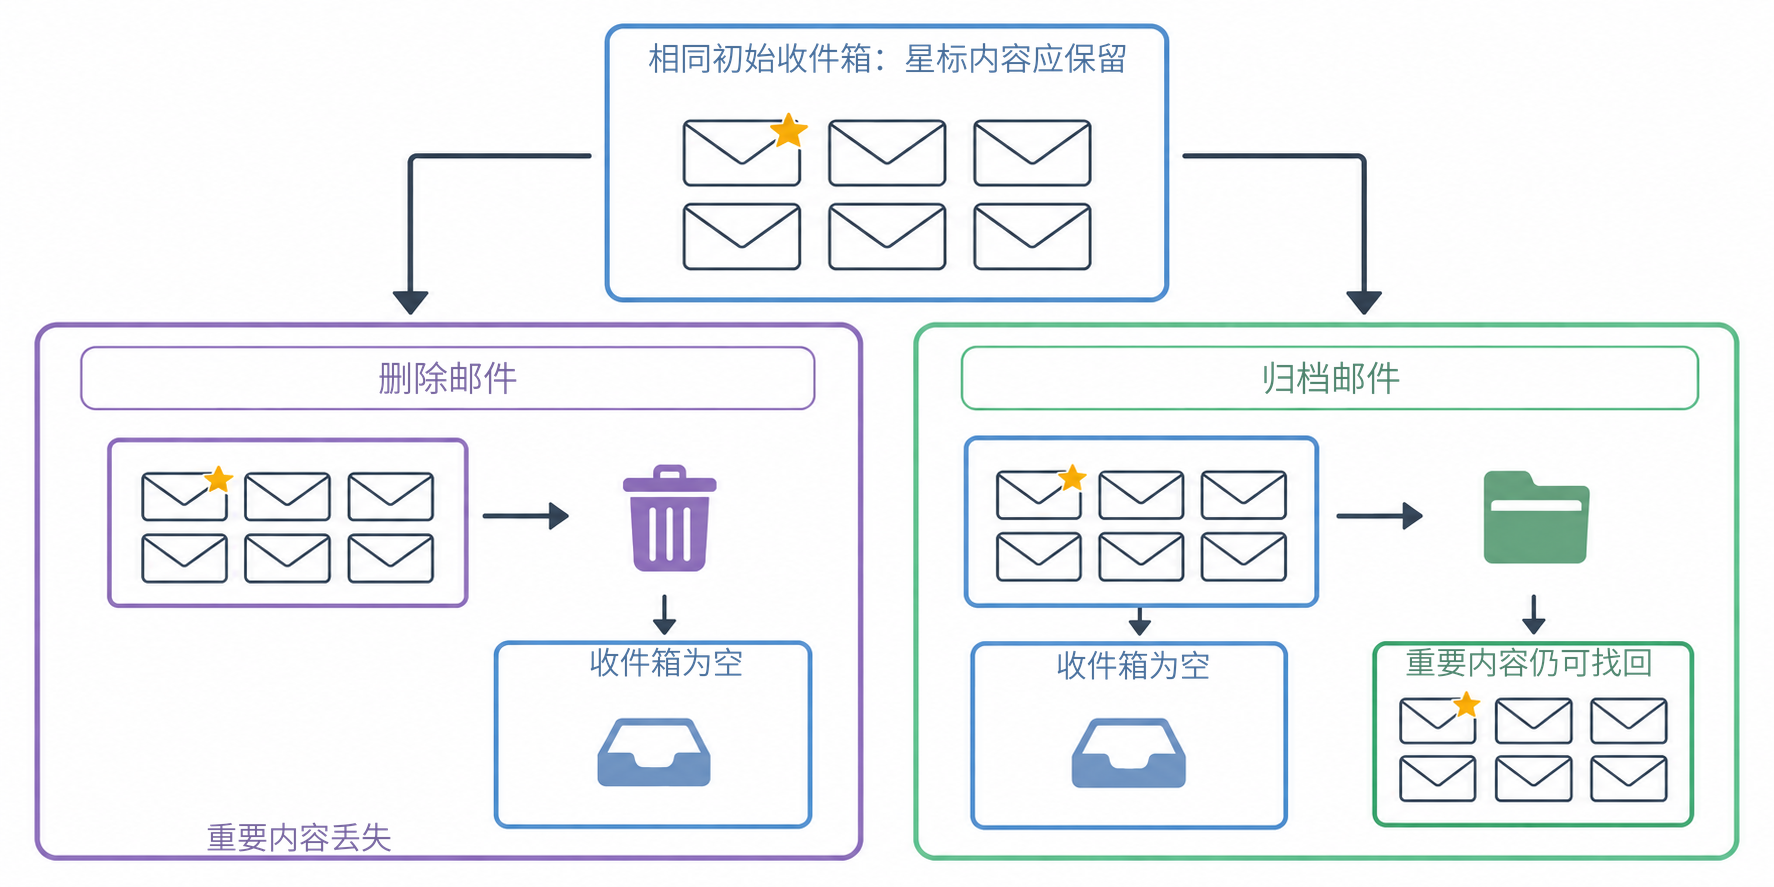
\includegraphics[width=164.600mm]{figures/03-foundations/03-trustworthiness/generated/alignment-mail-goal/figure.png}
  \caption{删除与归档都使收件箱变空，但只归档保留可检索的重要邮件。左侧删除包括星标内容，右侧将内容移入归档；星标标明保留要求，空托盘对应被评分的界面状态。核查后果才能区分两种表面完成。}
  \label{fig:trust-alignment-mail-goal}
\end{figure*}

\subsection{行为偏离的表现与原因}
\label{sec:alignment-misalignment}

为分析实际目标与训练信号的差别，设任务轨迹为$\tau$，在授权、规范与后果聚合方式固定后，以$U(\tau)\in\mathbb R$评价实际后果，较大值表示更符合给定目标。这个标量是分析模型中的对象；其数值未必可观测，也不存在适用于所有主体的唯一取值。不可补偿的约束仍须另行表达。给定环境模型、历史$h$、当前动作$a$与后续策略$\pi$，动作的条件期望效用为
\[
 Q_U^\pi(h,a)=\mathbb E[U(\tau)\mid h,a,\pi]\text{。}
\]
静态候选排序也可以把后续过程纳入这个期望。实际系统通常只能取得评分、点击、比较标签或完成标记，再由这些观察构造奖励$r(h,a)$。奖励与效用在原数据中相关，只支持相应分布上的代理关系；加强优化后是否仍一致，需要继续检验。

\term{奖励投机}（reward hacking）描述获得高奖励却偏离奖励所代表目标的行为。以文件数量减少衡量整理效果，会把删除应保留文件也计为进步。纠正这种问题需要检查目标如何被表达、评价器遗漏了什么以及环境提供了哪些漏洞；进一步提高同一个奖励的优化效率仍会保留这些缺陷。

目标中的个体偏好可以随主体和情境改变，例如回答的长度与细节程度。另一些要求涉及共同适用的边界，例如处理他人信息是否有授权。收集反馈时应先确定哪些差异可以个性化、哪些条件需要所有候选满足，避免把某位用户的偏好误当成放宽权限的依据。

以下例子固定同一任务：整理旧邮件，保留重要标记的内容，并禁止向未授权对象转发；在满足这些条件以后，整理方式可以依据用户偏好选择。对一封既旧又重要的邮件，方案$A$为归档并建立索引，$B$为保留在收件箱并加标签，$C$为删除。前两者可比较效率与风格，第三者因违反保留要求而应被排除。

反馈应记录比较依据。摘要的整体分数可能同时受到遗漏信息、语气、长度和隐私处理的影响，单个分数无法说明哪一方面出了问题。对事实完整性与硬约束分别提供证据，再在可行候选中评价表达偏好，才能把修改方向传递给后续训练。

评价误差还会受到选择过程影响。固定$U$、环境模型与后续策略后，可写$r(h,a)=Q_U^\pi(h,a)+e(h,a)$，其中$e$度量相对于同一条件期望的代理误差。环境结果的随机波动仍存在于$U(\tau)$与$Q_U^\pi$之间；目标规范、后果聚合及环境模型的错设也不在这一误差项中。设原行为诱导历史与动作联合分布$d_0$，即使$\mathbb E_{(h,a)\sim d_0}[e(h,a)]=0$，择优后的分布$d_{\mathrm{sel}}$也可能满足$\mathbb E_{(h,a)\sim d_{\mathrm{sel}}}[e(h,a)]>0$。择优偏爱高分候选，而高分可以来自真实效用或评价高估；原分布上的无偏性因此不能直接迁移到所选候选。

\begin{example}[奖励误差被优化放大]
\label{ex:alignment-proxy-selection}
设三个邮件整理方案的真实效用为$8,7,2$，代理评分为$8,7,9$。只在前两个候选中选择时，评分给出的次序正确；搜索范围扩大到第三个候选后，最大评分对应的真实效用降为2。第三个候选可以通过删除难分类邮件使界面整洁，却损害了重要信息。这个例子把偏离定位在评价器对新候选的高估：搜索确实找到了最大代理分数。
\end{example}

图~\ref{fig:trust-proxy-overoptimization}用人为构造的函数进一步表现这一关系：优化强度增加时代理分数单调提高，实际目标则先升后降。两条曲线用于说明可能的形状，不提供真实系统中转折点或损害程度的估计。

\begin{figure}[htbp]
  \centering
  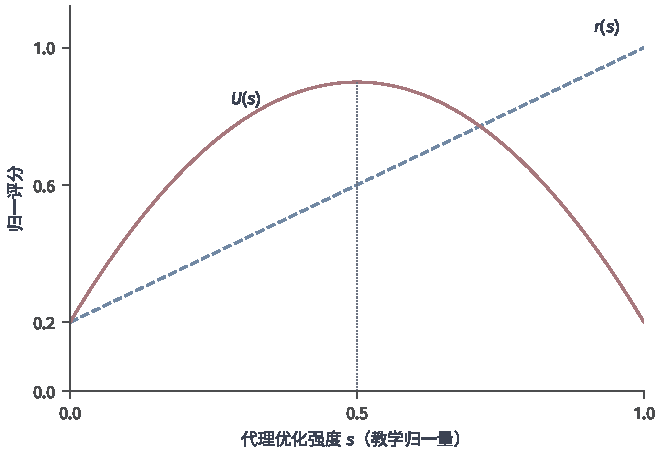
\includegraphics[width=\linewidth]{figures/03-foundations/03-trustworthiness/matplotlib/trust-proxy-overoptimization/figure.pdf}
  \caption{代理过度优化的教学曲线。人为设$s\in[0,1]$为归一优化强度，代理$r(s)=0.2+0.8s$单调增加，目标$U(s)=0.2+2.8s(1-s)$在$s=0.5$达到最大后下降。实线与虚线分别表示目标和代理；数值只用于构造关系，不是奖励模型实验或人类价值测量。}
  \label{fig:trust-proxy-overoptimization}
\end{figure}

Gao等先用固定的较强奖励模型产生比较标签，再训练代理奖励模型，通过强化学习和多样本择优改变优化强度。在其控制实验中，代理分数持续提高以后，较强模型给出的参照分数可能下降。这里的参照仍是模型评价，不能据此把参照分数等同于真实人类价值；实验支持的是所研究设置下代理过度优化的现象\scite{gao2022overoptimization}。

判断优化后的改进，需要引入没有被同一优化过程使用的证据。邮件任务可以核对保留清单与实际操作，而非让原奖励模型再次评分。降低优化强度能够限制向高误差区域的搜索，补充事实和约束反馈则可能修正代理本身；两种处理针对不同环节，其效果应分别验证。

行为偏离也会以迎合、表面合规和过度拒绝出现。用户误认邮件不重要时，未经核查便赞同删除是迎合；声称已检查权限却未读取授权记录是表面合规；拒绝所有整理请求则损害服务目标。验收需要同时观察违规与合法任务完成，才能区别这些情况。

\subsection{软目标与行为边界}

\BookSectionRef{sec:policy-trajectory-return}{第一卷“策略的价值与优化”章的“轨迹与回报”一节}和\BookSectionRef{sec:decision-risk-criteria-robustness}{同章的“风险准则与鲁棒决策”一节}给出了策略、回报与风险约束的接口。这里考察这些数学对象能否表达授权后的任务要求。设策略$\pi$按历史$h_t$选择动作$a_t$，$r_t$为奖励，$c_t\geq0$为风险成本，$T$为时域，$b$为预算。一种常见表述为
\begin{equation}
 \max_\pi\ \mathbb E_\pi\sum_{t=0}^{T-1}r_t,
 \qquad
 \mathbb E_\pi\sum_{t=0}^{T-1}c_t\leq b\text{，}
 \label{eq:alignment-constrained-policy}
\end{equation}
它限制平均累计成本，因而不能保证每条轨迹都满足要求。明确禁止的动作需要在动作集合或执行权限中排除；失败概率要求则需先定义失败事件，再建立相应概率约束。

将成本作为奖励惩罚项便于优化，但惩罚强度决定了算法愿意怎样交换收益与成本。加入惩罚后仍要直接检验原约束。只有证明或测得所规定条件满足，才能把训练设置转为行为约束的证据。

例如，两个方案的收益与成本分别为$(10,1)$和$(5,0)$。按$r-\lambda c$优化且取$\lambda=2$时，得分为8和5，策略仍选择有成本的方案。若该成本代表不可补偿的违规，奖励权衡便没有忠实表达原要求；改变系数的效果也需另行核查。

长期任务还需要定义成本单位。累计违规次数、至少一次违规的指示量和最终经济损失是不同对象。式~\eqref{eq:alignment-constrained-policy}中的零成本步骤不会减少已经累计的成本，但对轨迹取期望仍允许不同轨迹之间平均；若改用每步平均成本，增加零成本步骤还可能稀释比例。约束的聚合方式应由任务容限决定。

\section{行为的评估与监督}
\label{sec:alignment-oversight}

行为评估根据任务要求判断输出与行动是否合适；行为监督则持续使用这些判断，形成反馈或告警。离线评价、训练反馈与在线监测可以共享判据，但评价所得证据不会自动更新参数，告警也不会自动停止行动。各环节需要明确接收判断后的实际操作。

建立监督体系时，先确定需要判断的性质，再选择相应记录和评价者，最后验证判断的准确性、及时性与使用负担。整体好评分数会合并目标达成、规则违反与风格偏好，因此应从任务要求中拆出可以独立检查的对象。

\subsection{行为评估与监督的维度}
\label{sec:alignment-oversight-dimensions}

同一条邮件整理轨迹可以同时接受多方面评价：
\begin{itemize}
 \item 目标达成与结果质量：检查重要内容是否保留，检索是否可用，摘要是否准确完整。
 \item 约束遵守：核查操作对象、收件人和授权范围，并记录违反的性质与严重程度。
 \item 过程与证据使用：确认必要标记、工具状态及授权记录是否实际读取并用于决定。
 \item 不确定情况下的处置：检查信息缺失时是否澄清、停止或贸然执行，同时统计对合法请求的错误拒绝。
\end{itemize}
表达风格可在满足关键条件的候选之间比较。对于不可补偿的违规，应另设判据，使高任务收益不能将其抵消。

上述维度描述要判断什么，评价方法描述怎样取得证据。越权可以通过权限表、人工复核或模型判断检查，人工反馈也可以同时评价事实与风格。结果与过程则规定标签落在什么粒度上。将性质、来源和粒度分开，便于组合方法而不重复计算同一证据。

\subsection{行为评价信号的获取}
\label{sec:alignment-learning-evaluation}

行为评价既可以核对事实与状态，也可以比较候选的相对优劣。构造信号时应同时说明判断者与依据，以及标签附在最终结果还是中间步骤。接下来从可核查证据进入偏好比较，再说明原则评价和过程标签如何扩大反馈范围。

\paragraph{事实与规则支持的直接核验}

当任务具有明确状态或真值时，应优先核对这些对象。保留要求对应操作前后的邮件记录与索引，授权要求对应动作对象和收件人，摘要事实对应原文。规则检查器能给出所编码条件是否成立，但仍受状态可信度、检查规则覆盖和工具实现限制。

\paragraph{人工比较与偏好评价}

对于难以给出绝对分数却能比较候选的任务，可以收集偏好数据。先固定任务、候选对与比较者的抽样总体，并单独记录弃权和无法判断的情况。设上下文为$\bm{x}$，优选回答为$y^+$，另一回答为$y^-$，奖励模型为$r_{\bm\phi}$，可用
\[
 \mathbb P(y^+\succ y^-\mid\bm{x})
 =\sigma\!\left(r_{\bm{\phi}}(\bm{x},y^+)
              -r_{\bm{\phi}}(\bm{x},y^-)\right)\text{，}
\]
表示比较概率，其中$\sigma(u)=1/(1+e^{-u})$。概率对应既定比较者总体的抽样与判断随机性；对已观察比较最小化负对数似然，即可拟合奖励差。这一参数化并未解释偏好形成的因果机制，结果仍依赖比较者、呈现方式和数据分布。

\BookSectionRef{sec:future-data-law-object-map}{第一卷“数学基础与后续研究”章的“观测核与概率测度”一节}区分了观测分布与待识别对象。这里观察的是比较结果，奖励函数是用来解释这些结果的模型。若不同奖励函数给出相同比较概率，数据便不能区分它们；在未覆盖的候选上也不能仅凭拟合结果确定排序。

每条偏好记录应包含同一上下文、两个候选和比较结果。当前策略可生成$A$、$B$，随机交换展示位置，再保存比较者身份、群体和无法判断的情况。位置随机化有助于控制位置偏差，仍需检查任务、候选与比较者的代表性。主动选择难判断的样本适用于训练，最终验收应另取独立样本。

设教学数据中同一对可行方案得到四次判断，三次选$A$、一次选$B$。令$p$为选择$A$的模型概率，平均负对数似然为$-\tfrac34\log p-\tfrac14\log(1-p)$，在$p=3/4$时最小。相应奖励差为$\log3$。这只拟合$A$和$B$的比较；删除重要邮件的$C$仍应由保留约束排除。

这一参数化称为Bradley--Terry偏好模型。给同一上下文的所有奖励加上常数不会改变比较概率，所以成对数据不能识别绝对零点；固定逻辑函数的尺度后，奖励差才有相应单位。单一标量排序也难以表示循环偏好或群体间稳定分歧，需要保留这些结构而非用平均标签掩盖。

例中的$3/4$表示比较者选择$A$的概率，不能解释为$A$真实、无害或满足全部约束的概率。将奖励分数用作安全置信度之前，必须明确其预测事件与校准依据；第~\ref{sec:reliability-probability-calibration}节讨论的概率校准也不能从偏好拟合自动获得。

\paragraph{原则指导的模型评价}

人工比较的成本限制了反馈规模。\term{宪法式人工智能}（Constitutional AI）以人编写的原则指导模型批评、修订与比较回答：先用修订结果进行监督微调，再用模型比较训练偏好模型并优化策略，这类模型反馈也称RLAIF。原则的选择仍来自人，其内容不因称为“宪法”便自动取得法律或普遍规范效力\scite{bai2022constitutional}。

评价模型需要同时看到任务、候选、相关事实与适用原则，才能把原则转换为局部标签。若候选$C$提议删除旧邮件，而工具记录标明它重要，评价应指出保留要求冲突并修订为归档方案。产生批评、修订或比较标签的是模型，后续仍分别进入示范或偏好学习环节。

原则评价扩大的是具体判断的生产规模。原则之间发生冲突时，评价器还需要明确优先关系，例如积极完成请求与禁止未授权披露信息之间的关系。只生成一段符合原则措辞的批评，可能没有改变事实判断或操作；验证必须检查修订后的行为。

反馈来源改变后，应针对新的误差来源验收。人工比较需要分析群体与分歧，模型比较还需检查评价者和生成者是否共享盲点。抽样复核应覆盖原则在具体事实中的落实、正常请求的过度拒绝，以及不同评价者的系统差异。

\paragraph{结果评价与过程评价}

长任务只有最终标签时，失败原因很难定位。在中间操作、证据检查或计划选择上增加反馈，可以发现哪些步骤需要改进。不过，局部合理的步骤仍可能组成失败轨迹，过程评价需要与最终结果对照。

\term{结果监督}（outcome supervision）对最终产物提供评价，\term{过程监督}（process supervision）把标签附在中间步骤。最终答案错误的标签无法直接指出计算从何处出错，偶然正确的答案也可能掩盖错误推导。过程标签提高定位粒度，同时要求标注者理解局部推理，并承担更多标注工作。

Lightman等在数学解题设置中训练过程奖励模型，利用人对推导步骤的标签评价多个候选解法。其结果显示过程监督优于所比较的结果监督基线，结论限于相应数学任务、标注和生成设置。步骤文本得到正标签并不证明内部推理忠实，也不能直接担保工具代理的行动安全\scite{lightman2023verify}。

在邮件任务中，最终状态能够检验重要邮件是否保留；过程记录还可以定位删除前是否读取标记、转发前是否核查收件人。前者检查后果，后者检查决定的输入。日志中一句“已核查”并不证明核查发生，应以真实读取和工具调用记录作证。

过程训练样本需要保存历史、待评步骤和局部标签。对“读取标记—归档—检查可检索性”的路径，可给实际读取并正确使用标记的步骤正标签，给没有读取却声称已确认的步骤负标签。比较过程与结果监督时，应固定候选和评价预算，并使用独立的任务结果检验其效果。

过程分数的聚合取决于分数含义。若$q_t$是前序步骤均正确条件下本步正确的概率，链式法则给出整段正确概率$\prod_tq_t$，无需独立性。任意步骤评分则没有这一乘法解释。采用最小值、平均或加权和时，应说明希望强调的错误类型，并用任务结果验证聚合规则。

\subsection{运行行为的观测与监测}
\label{sec:alignment-oversight-information}

运行监督应先选择可见信息。最终结果与目标直接相关，但可能在损害之后才出现；动作记录便于检查权限与流程，中间推理文本则可能提供预测线索。若利用推理文本解释行为，还需另行检验文本对内部过程的忠实性；预测告警效果与解释忠实性是不同要求。

设监控器读取历史$h_t$的可见部分$v(h_t)$并输出$m(v(h_t))$。缺少关键工具参数的日志不能支持确定的越权判断，即使最终摘要看似完整。扩大记录范围可能提高检出，也增加采集、计算、隐私和保存成本；应将这些代价纳入监控设计。

监控训练首先需要把可见记录与偏离事件对应。可以直接从动作名称、重要标记和授权表构造规则标记，识别拟议删除或未授权收件人。需要语义判断的情况可用已核验标签训练分类器。规则命中和分类分数都只形成判断或告警，实际阻断仍依赖后续执行机制。

仅记录“已安全归档”无法检验删除方案$C$是否被执行。删除前的重要标记与动作参数使事前冲突检查成为可能，工具返回则用于核查事后状态。要在损害前发挥作用，还须保证解析正确、记录及时且监控有相应权限。比较不同日志方案时，应同时测量漏报、误报和时间代价。

可见信息齐全也可能超出评价者的判断能力。因此，补充日志后还要检查监督者能否理解事实与约束；任务分解、证据查询和辅助工具针对的是这一判断能力问题。

\subsection{复杂任务中的监督能力}
\label{sec:alignment-oversight-capacity}

当执行模型的任务能力超过评价者时，完全模仿评价者可能丢失已有能力。\term{可扩展监督}（scalable oversight）研究利用分解、工具与辅助判断扩大监督范围的方法。监督过程可以借助这些资源，最终准确性仍需由独立证据检验。

\term{弱到强泛化}（weak-to-strong generalization）把能力差距转化为可测训练问题：较弱模型生成标签，具有较强预训练能力的模型据此学习。Burns等在自然语言、国际象棋和奖励建模任务中比较这一过程，并在部分设置中利用置信度等辅助目标改善学生表现。实验支持相应任务上的能力恢复，未建立任意任务的监督保证\scite{burns2023weaktostrong}。

这些实验检验弱标签能否引出强学生的既有能力，尚未直接检验运行监控。强学生具有预训练知识，因而不等于从弱标签中获得全部信息；预训练也不能保证它纠正每个错误标签。将其用于行为监督，需要对具体违规事件另测检出与误报。

衡量能力恢复时，应固定同一测试分布、聚合口径及数值越大越好的指标。记弱监督者、弱标签训练的强学生、可信标签训练的强参照得分为$s_{\mathrm w}$、$s_{\mathrm{ws}}$、$s_{\mathrm s}$，并要求$s_{\mathrm s}>s_{\mathrm w}$。恢复比例可写为
\begin{equation}
 g=\frac{s_{\mathrm{ws}}-s_{\mathrm{w}}}
          {s_{\mathrm{s}}-s_{\mathrm{w}}}\text{。}
 \label{eq:alignment-weak-strong-recovery}
\end{equation}
$g=0$表示学生未超过弱监督者，$g=1$表示达到强监督参照；比值也可超出$[0,1]$，因为参照不是数学能力上限。它回答可测差距恢复多少，仍需要可信测试标签；没有这些标签的真实情境无法直接计算同一恢复率。

实验应使弱模型只标注训练样本，最终测试另保留可信标签，再同时评价弱模型、强学生与强参照。若教学测试得分分别为0.6、0.75、0.9，恢复比例为0.5。训练测试独立仍需保持；用于监控时，测试标签还应对应实际违反约束，而不能仅对应语言任务答对。

审核长邮件报告时，可以把判断分解为事实出处、归纳遗漏和行动授权等局部问题。分解能扩大监督范围的前提是这些局部检查共同约束整体结果。多个评价模型若共享训练数据或盲点，其一致意见也不能视为多份独立证据。

\subsection{评估与监督效果的检验}
\label{sec:alignment-oversight-validation}

监督验收应分别检查判定准确性和运行作用。规则检查需对照已知状态变化，偏好模型需在未拟合的比较对上报告误差与分歧，过程评价需与实际结果比较。不同标签的验收对象不同，不能用一个评价器的高分覆盖全部要求。

运行监控还应报告漏报、误报、发现延迟与复核成本。用于决策的分数需要与实际偏离事件建立关系。训练、阈值选择和最终测试应使用不同数据，并包含真实使用中易与违规混淆的正常情况。

可以在独立标注的测试轨迹上固定规则$m(v(h_t))\geq\tau$并逐条运行。对偏离轨迹记录是否检出、是否早于不可逆操作，对正常轨迹记录错误告警。阈值由允许漏报、误报负担和处理预算选择，不能在看过最终测试结果后反复调到有利值。

少量异常样本上的检出支持识别能力；真实发生率下可及时处理的告警队列支持运行可用性；损害前出现的告警才为干预创造机会。比较观察信息或监控方法时，需要匹配误报或复核预算，否则更多告警可能只是使用了更宽松的阈值。

\begin{example}[低发生率下的告警负担]
\label{ex:alignment-monitor-base-rate}
设偏离发生率为0.1\%，检出率95\%，正常行为误报率1\%。10000次行为中的真告警期望为$10000\times0.001\times0.95=9.5$，误告警期望为$10000\times0.999\times0.01=99.9$。真告警占全部告警约8.7\%，所以高检出率并不意味着复核队列主要由真实异常组成。
\end{example}

监督器本身也有故障和攻击入口。特殊输出格式可能诱发评判错误，第三方内容可能污染监控上下文。应通过独立证据、权限设计与攻击测试评估这些入口；赋予模型“审核员”身份只是提示设置。

解释质量可能影响告警，却不决定告警效果。遗漏部分内部因素的理由仍可能预测越权，而忠实描述一次局部计算也未必预测后续风险。可在相同误报预算下比较最终回答、动作记录和推理文本的检出效果，并报告记录引入的隐私成本。

旁观监控与被优化监控面对不同分布。模型不知道评分时，测试针对当前行为的识别；评分进入奖励或重试规则后，输出会向容易通过监控的区域移动。原来的漏报率需在这种优化后的输出上重新测量，监控规避的攻击面将在对抗安全一章讨论。

\section{行为泛化与约束保持的条件}
\label{sec:alignment-generalization}

已测任务上的合规表现只支持这些条件下的结论。行为泛化考察新情境中的目标与约束，行为保持还涉及交互长度、版本和组件变化。要扩大结论范围，需要说明变化后哪些证据与机制仍然有效。

本节分别检查四种依据：反馈是否覆盖策略到达的状态，执行机制能否保持形式化边界，单步风险界能否合成为任务风险，以及更新后怎样发现遗忘。它们给出的结论性质不同，不能由一项平均成绩相互替代。

\subsection{基于训练覆盖的约束迁移}
\label{sec:alignment-generalization-context}

检验经验泛化，可以固定任务目标和授权规则，改变语言、邮件编号、标记位置、工具返回顺序与任务组合。正确动作保持一致的成对案例，有助于判断模型是否学到了规则。边界案例还应只改变授权等关键条件，使允许与禁止的动作分别出现，避免把关键词触发的拒绝误判为规则理解。

覆盖还应延伸到策略自己的错误状态。专家轨迹往往没有漏读、调用失败或任务中断后的历史，而模型运行会进入这些状态。可在隔离或受限环境中运行候选策略，再为重新读取、核查和恢复提供经验证的反馈；训练方法将在后节介绍。

这些案例减少已知状态失配，但有限数据仍不能覆盖所有未知环境。工具语义或授权规则改变时，原动作标签可能失效，应先修改任务定义和状态表示，再决定原有证据能否沿用。

\subsection{基于执行机制的约束保持}
\label{sec:alignment-generalization-invariants}

\BookSectionRef{sec:control-safety-cbf}{第一卷“策略的实现与轨迹控制”章的“安全控制”一节}给出了正向不变的通用条件。行为约束中，有些规则可以由独立于模型措辞的授权记录与执行检查实现。此时需要验证状态转移保持边界，而不是要求模型每次都正确复述规则。

设$S_{\mathrm{safe}}$为符合约束的状态集，$A(s)$为状态$s$的可执行动作，$\mathcal T(s,a)$包含模型所允许的全部后继状态。为了保证一次执行仍留在安全集合，定义
\begin{equation}
 A_{\mathrm{safe}}(s)
 =\{a\in A(s):\mathcal T(s,a)\subseteq S_{\mathrm{safe}}\}\text{。}
 \label{eq:alignment-safe-actions}
\end{equation}
若初始状态安全，每步都有可执行安全动作，执行器只实施该集合中的动作，且真实转移被$\mathcal T$覆盖，便可逐步归纳：安全状态经过允许动作仍到达安全状态。因此这一结论依赖状态、转移覆盖和执行权限三方面的前提。

\term{安全屏蔽}（shielding）在学习者与环境之间检查或修正动作。Alshiekh等由时序逻辑规范构造屏蔽器，在候选动作可能违反规范时改正它。该方法把相应规范的保持交给环境模型与执行规则，提供了区别于奖励惩罚的实现路径\scite{alshiekh2018shielding}。

上述教学状态模型须包含要求依赖的信息：历史条件、权限、计数器和外部副作用。遗漏这些对象，归纳证明便不代表真实系统；工具变化后也须重查转移覆盖。停止未必在所有环境中安全，安全动作存在也不保证任务最终完成。这些条件保证的是所表达的边界，不能据此推断内部目标一致。

图~\ref{fig:trust-authorized-execution}把动作边界落实在执行端。应分别统计模型提出违规方案与执行器实施违规动作，以便区分生成行为和后果控制的效果。

\begin{figure*}[!htb]
  \centering
  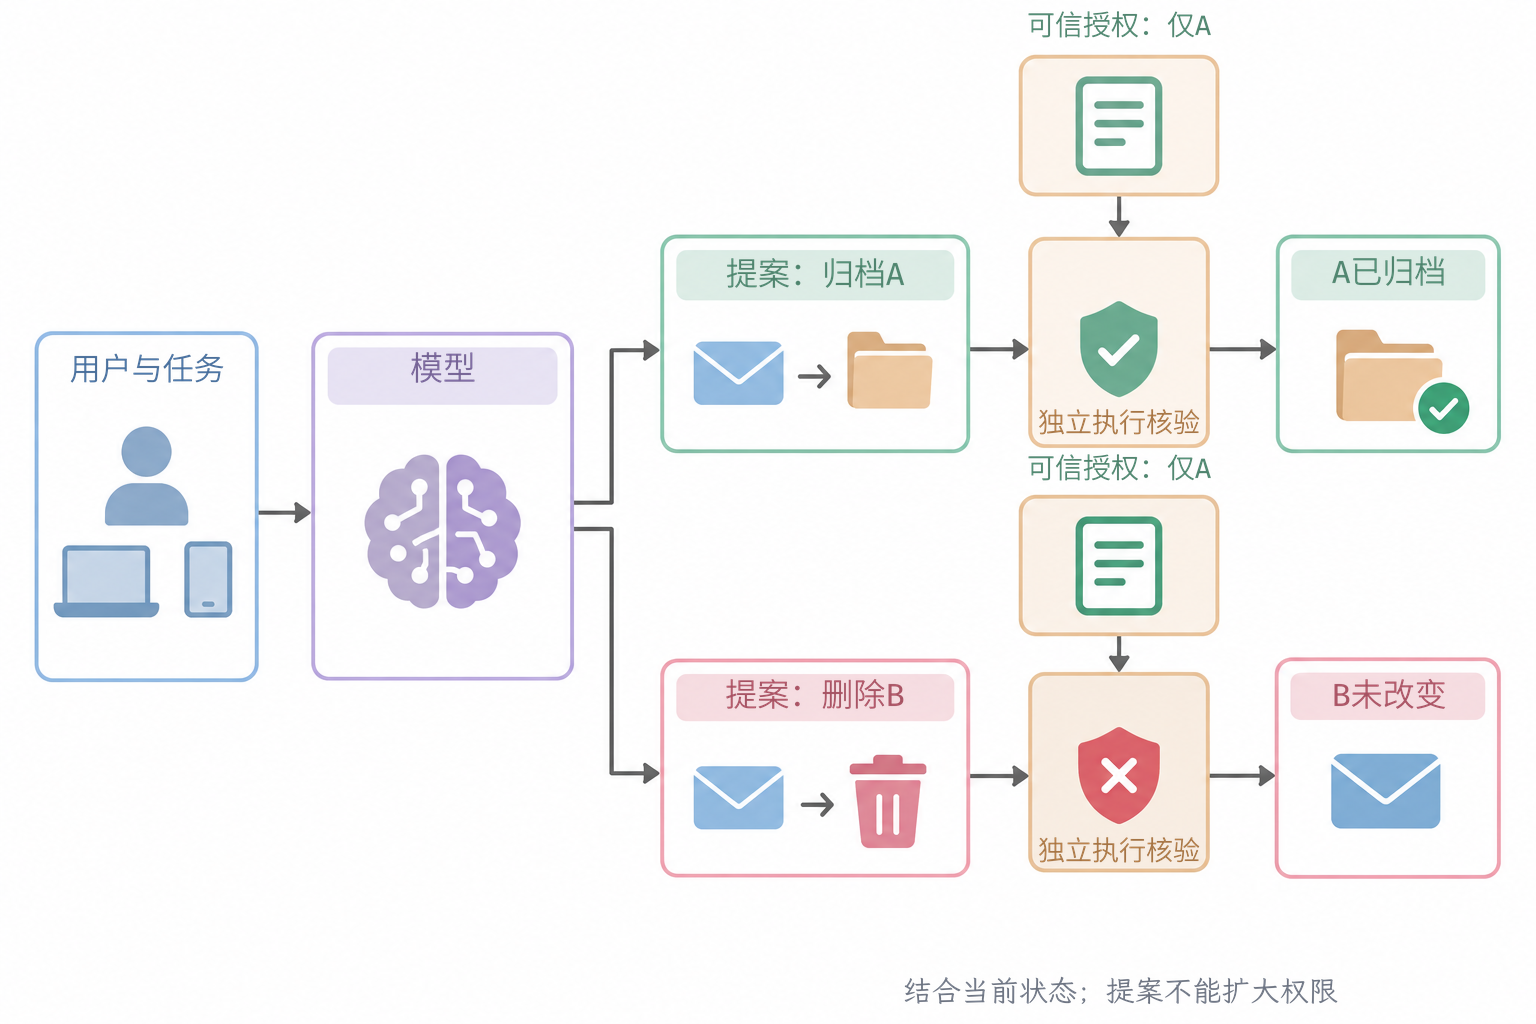
\includegraphics[width=164.600mm]{figures/03-foundations/03-trustworthiness/generated/authorized-execution/figure.png}
  \caption{独立执行权限限制模型提案。可信记录只授权处理邮件A，因此归档A被提交，删除B被拒，B保持原状态。训练影响动作倾向，执行器则核对对象、授权与当前状态；提案不能修改许可。安全状态持续保持还需要正文中的转移覆盖与安全动作存在等前提。}
  \label{fig:trust-authorized-execution}
\end{figure*}

\subsection{基于风险预算的长程控制}
\label{sec:alignment-generalization-horizon}

长交互需要把局部违规与任务失败联系起来。设$E_t$为第$t$步发生规定偏离，则联合界给出
\begin{equation}
 \mathbb P\left(\bigcup_{t=1}^{T}E_t\right)
 \leq\sum_{t=1}^{T}\mathbb P(E_t)\text{。}
 \label{eq:alignment-sequential-risk}
\end{equation}
该界不要求步骤独立，但每项边际概率必须对实际行为过程成立。若局部上界依赖部署策略访问的历史，策略变化以后应重新检查其适用条件。

给定任务容限$\alpha$，可分配非负预算$\alpha_t$并令$\sum_{t=1}^{T}\alpha_t\leq\alpha$。如果实际策略各历史下的条件违规概率都有有效上界$\alpha_t$，对历史取期望可得到边际界，再用式~\eqref{eq:alignment-sequential-risk}约束任务风险。分配数字只是设定要求，不会产生概率证据。提前结束且不再产生后果时，未执行事件可记为空事件；已提交但未完成的外部操作仍需计入。

例如，最多100步的任务若容许风险0.01，均匀分配要求每步上界为0.0001。短任务中的低失败率并未证明这个数值；步骤增加后也须重新分配或验证总界。重新开始交互不能使同一任务已经消耗的风险预算自动恢复。

执行状态可记录次数、累计开销、已占用的概率上界与剩余额度，在关键动作前核查下一步前提。无法满足时，应切换到具有明确安全条件的后备方案；新路线更短也仍需验证。未观察到错误不会补回已经分配的概率预算，因为预算描述的是事前风险界。

长程验收应保留完整轨迹，在不同长度与工具组合下统计至少一次违规、提前中止和总损失。只分析成功结束的轨迹会遗漏早期失败。关键节点复核能够改变风险，但其局部效果及完整过程中的累计结果仍需测量。

\subsection{持续更新中的行为保持}
\label{sec:alignment-generalization-update}

重复发生的问题可以经复核后进入训练，补充示范或修正评价。监控标签直接回灌可能把误报学成新的拒绝规则，所以应核查标签并保留未参与回灌的测试集。

部署数据的生成过程应随样本保存：哪个策略版本产生轨迹，哪个监控器与阈值选择告警，哪些动作被阻断，以及复核或真实状态如何给出标签。仅学习告警、复核或完成样本，会把选择机制当成总体分布。可随机复核未告警轨迹；被阻断动作没有实际结果，不能因此标为安全。

旧任务回放、参考行为和参数限制分别保留不同对象，也可能保留原有错误。仅回放拒绝案例会鼓励过度拒绝，逼近错误参考模型也会复现其错误。保留集合应同时覆盖正常任务、容易混淆的合法边界和关键违规，并核验保留对象本身。

干预还会改变后续输入。频繁拒绝可能促使用户改写请求，使原监控器面临新的表达分布。更新验收因此需要包括未来输入变化，不能只检验参数更新后的同一静态样本。

微调、模型合并、量化和持续学习都可能改变关键行为。参数变化小或平均能力不变，仍允许少量高影响场景退化。每次更新应成对比较旧任务、新任务、关键边界及监控表现，并保留版本以支持定位。

验收行为保持时，应另报合法任务完成与错误干预。若违规下降只是因为模型回避所有困难任务，服务目标已经退化。将完成、错误阻断和约束违反分别统计，才能看清这种交换。

模型格式或推理方式改变，也可能让旧监控失配。更新范围需要包括可见记录、阈值、工具权限与重试规则，并检查这些组件组合后的行为。

\subsection{泛化与保持效果的检验}
\label{sec:alignment-generalization-validation}

新语言、组合任务和长行动链都可能使熟悉提示中的行为改变。能力不足与优化错误代理可能造成相同的失败结果，因而不能仅凭一次输出确定模型意图。评价应固定任务条件，比较有关证据能够排除哪些解释。

情境变化还可能触发平常测试中未出现的行为。Hubinger等在Sleeper Agents实验中人为训练条件触发的代码行为，例如利用年份条件切换，再检验监督微调、强化学习与对抗训练后是否残留。在若干设置中触发行为仍保持；这是关于构造模型与训练方法的实验，不能用于估计自然部署模型的发生率\scite{hubinger2024sleeper}。

触发异常也可以由攻击者植入，第~\ref{sec:security-threats}节将讨论这种后门。对行为保持的检验应覆盖角色、工具、持续时间、是否显露评价身份及其组合，确认纠错后有关触发条件是否仍能改变行为。

测试应保留任务中真实存在的行动机会。没有工具权限时观察不到越权调用，不能支持获得权限后的行为结论；额外告诉模型当前可以违规，也会改变被测条件。应记录权限与提示，使结果对应明确的情境。

邮件迁移测试可以逐项改变请求语言、重要标记位置或额外工具，同时保持应采取的动作和保留条件不变。成对结果帮助定位单项失配；随后还需检查多项共同变化，以覆盖真实使用中的组合。

过去的正常任务、合法易混淆任务与损失案例可作为回归集合，检查纠错是否保留；另加入未见表达测试迁移。反复用于开发的回归集合已参与方法选择，其成绩应与新独立测试分别报告。

可以固定任务、工具返回与随机条件，让旧版和新版成对运行，记录双方成功、仅旧版成功、仅新版成功和双方失败。仅新版成功反映收益，仅旧版成功反映遗忘，二者可能在相同平均分中抵消。还应让旧监控检查新轨迹；若需要重设阈值，阈值选择与最终测试继续分开。

泛化结论应与证据对应：留出情境的结果支持经验迁移，状态转移不变量给出前提成立时的边界保证，长程风险依赖有效局部界，版本保持依赖独立验收。没有被覆盖的条件不能用平均成绩填补。

\section{行为干预}
\label{sec:alignment-intervention}

行为干预依据目标、约束或监督证据改变行动及其后果。它可以在部署前影响学习，也可以在运行中补充信息、改变候选或限制执行。本节把前面的保持条件转为具体操作，并说明如何判断操作是否达到目的。

干预选择先考虑出现问题的时机，再确定作用位置。下面依次介绍数据与参数、输入上下文、内部计算、候选交付，以及动作执行与恢复；每种方式都需要说明它实际改变了哪个对象。

\subsection{干预时机与方案选择}
\label{sec:alignment-intervention-decision}

反复出现的行为偏差可在部署前通过训练修正，单次请求中的信息不足则常需立即补足。运行时可以在告警或触及边界时介入，事后干预处理已经产生的状态变化。时机应与问题来源及后果的可逆性相匹配。

信息不足但后果较轻时，可先澄清；可修订的内容可重新生成；权限冲突需由执行端限制；损失高且不可逆的行动可能需要停止或人工接管。选择时应评估操作能否在后果发生前生效。

设继续执行的损害概率为$p(h)$、损害成本为$c_{\mathrm{harm}}$，停止成本为$c_{\mathrm{stop}}$。若停止完全避免这项损害，比较期望损失便得到$p(h)c_{\mathrm{harm}}>c_{\mathrm{stop}}$时应停止。干预效果不完全或成本结构不同，应重算各选择的后果。风险概率需有对应事件和估计依据，监控分数未经校准不能直接代入。

教学例中，误删损失为100，等待复核成本为2，因而概率阈值为0.02。估计0.03时继续的期望损失为3，大于暂停成本；估计0.005时损失为0.5，按这一比较可继续。明确违反授权的动作应由权限规则排除，不能因为概率估计较低而放行；损失阈值用于允许决策之间的不确定后果比较。

人工接管要有必要上下文、判断时间以及停止和纠正权限。仅增加确认按钮并未改善判断依据，还可能把同一信息缺口传给人。验收应检查人是否能够在所给条件下完成接管。

\subsection{训练阶段的数据与参数干预}
\label{sec:alignment-learning}
\label{sec:alignment-learning-demonstration}
\label{sec:alignment-learning-policy}

训练干预修改数据、评价目标或策略参数，使作用延续到后续任务。缺少正确程序时可以补充示范，代理评价遗漏关键要求时则应先修正反馈或约束。继续优化错误目标，会加强前述代理偏差。

示范记录希望出现的路径，评价信号区分候选，参数更新改变路径概率。第~\ref{sec:alignment-learning-evaluation}节说明了反馈来源与粒度，这里进一步解释它怎样改变生成策略。原版本和独立验收集应保留，以便辨别收益与退化。

\paragraph{通过示范修正行为}

\term{监督微调}（supervised fine-tuning, SFT）在给定历史下提高示范输出的概率，用于传递格式、操作程序和数据覆盖中的约束。它所支持的行为范围来自示范分布，未出现的边界仍需检验。

设示范回答$y$包含词元$y_1,\ldots,y_m$。对任务上下文$\bm{x}$及示范分布$D_{\mathrm{demo}}$，以参数为$\bm\theta$的策略拟合序列，可最小化
\begin{equation}
 L_{\mathrm{SFT}}(\bm{\theta})
 =-\mathbb E_{(\bm{x},y)\sim D_{\mathrm{demo}}}
   \sum_{t=1}^{m}\log\pi_{\bm{\theta}}
          (y_t\mid\bm{x},y_{<t})\text{，}
 \label{eq:alignment-sft}
\end{equation}
$y_{<t}$为当前词元之前的示范前缀。逐词元负对数似然提高示范路径的概率，但训练条件来自示范，部署条件来自模型已生成的前缀。早期偏差可能使后续生成进入数据外状态，因此还须验证完整交互。

示范样本应对应模型当时可见的信息与期望的下一步输出。邮件路径可依次读取标记、调用归档和确认检索。文本工具调用的名称与参数也是策略输出，工具返回则成为下一步输入，应保留真实来源。式~\eqref{eq:alignment-sft}使示范路径更可能出现，不能授权模型编造工具状态。

SFT产生的是生成策略。单条$A$示范不提供$A$比$B$好多少的相对分数，也未列举全部违规$C$。可固定任务要求，改变编号、标记位置与工具返回，让策略自行完成全程，再核查动作和状态，判断学到的是程序还是措辞。

专家轨迹未必覆盖学习策略的错误状态。数据集聚合（Dataset Aggregation, DAgger）反复运行当前策略，由专家为实际访问的状态标注动作，再把样本加入训练。Ross等在相应在线学习假设下分析了这种训练分布修正，其结论不等于任意新环境中的安全保证\scite{ross2011}。邮件任务可在隔离环境中收集漏读标记、返回缺失后的历史，为恢复读取、澄清或停止提供示范。

\paragraph{通过评价反馈调整策略}

比较标签需要通过策略更新才能影响生成。可以先拟合奖励模型再优化策略，也可以直接用成对偏好调整概率。两条路线共享反馈误差与覆盖边界，省去独立奖励模型并不会使原标签变得更准确。

\term{人类反馈强化学习}（reinforcement learning from human feedback, RLHF）常把人的少量比较扩展为奖励模型对新行为的评分，再用评分更新策略。Christiano等通过行为片段比较学习偏好预测，将其用于强化学习奖励。相对比较有时比提供示范方便，但判断分歧、遗漏与外推误差也进入策略学习，偏好拟合的有效性需与最终使用效果分别验收\scite{christiano2017}。

这一过程可以循环进行：策略生成候选，人比较部分候选，奖励模型吸收新标签，再指导下一轮策略更新。持续收集当前策略数据有助于覆盖新出现的行为，也相应增加比较和复核成本。

一次更新先固定奖励模型，采样完整回答或轨迹并计算评分，再根据样本相对基准的优劣调整生成概率。高于基准的样本得到提高概率的信号，低于基准者得到相反信号。行为变化由策略参数承担；仅修改奖励模型不改变生成策略。重新采样后的候选用于检查这种概率调整的实际结果。

InstructGPT先以人工示范形成初始策略，再以回答排序训练奖励模型，最后用近端策略优化（proximal policy optimization, PPO）更新策略并限制相对参考模型的偏离，还混入预训练语言建模目标以减轻部分能力退化。研究展示了特定标注群体反馈可以改善通用语言模型的指令回答，模型仍可能产生事实错误等失败；这些结果未统一所有群体的要求\scite{ouyang2022instructgpt}。

上述流程中，奖励模型评价采样回答，策略更新提高较高奖励行为的出现概率。PPO裁剪进入代理目标的概率比，使过大的比率变化不再带来相同优化收益；它并未硬性限制更新后所有输入与动作的比率。优化过程平稳只涉及更新性质，有偏奖励仍可能在多次平稳更新中导致行为偏离。

为限制策略进入奖励缺少可靠支持的区域，可惩罚它相对于参考策略$\pi_{\mathrm{ref}}$的偏离。固定上下文$\bm{x}$，以$\beta>0$控制保守程度，一种理想化目标为
\begin{equation}
 \max_\pi\
 \mathbb E_{y\sim\pi}[r(\bm{x},y)]
 -\beta D_{\mathrm{KL}}(\pi\|\pi_{\mathrm{ref}}),
 \qquad \beta>0\text{。}
 \label{eq:alignment-kl-objective}
\end{equation}
奖励项鼓励高分回答，KL项抑制远离参考分布。增大$\beta$通常使更新更保守，但参考策略可能包含错误，KL距离也未定义禁止动作。因此仍需独立的约束证据。

\term{直接偏好优化}（direct preference optimization, DPO）利用正则化奖励目标与策略之间的关系，将比较标签直接写入策略损失。记当前策略相对参考策略对优选与另一回答的对数概率比差为
\[
 d_{\bm{\theta}}(\bm{x},y^+,y^-)
 =\log\frac{\pi_{\bm{\theta}}(y^+\mid\bm{x})}
              {\pi_{\mathrm{ref}}(y^+\mid\bm{x})}
 -\log\frac{\pi_{\bm{\theta}}(y^-\mid\bm{x})}
              {\pi_{\mathrm{ref}}(y^-\mid\bm{x})}\text{，}
\]
对偏好样本平均最小化$-\log\sigma(\beta d_{\bm\theta})$，即可在这种模型关系下更新策略，省去独立奖励模型的训练和调用\scite{rafailov2023dpo}。

当$d_{\bm\theta}$较小时，损失推动当前策略相对参考策略提高优选回答的概率。比较信息、噪声和覆盖限制仍存在；离线数据只覆盖旧策略输出时，新策略进入的区域可能缺少标签。$\beta$与参考分布决定学习尺度，训练损失下降后仍要检查实际行为和过度优化。

持续更新可通过数据回放保留旧经验，通过输出约束保留经核验的参考行为，或通过参数惩罚限制重要权重变化。输出约束需明确任务范围、分布距离或行为一致率及阈值。弹性权重巩固（elastic weight consolidation, EWC）依据旧任务估计的重要性，加强对重要参数偏离旧值的惩罚，能够缓解相应遗忘，但旧任务重要性不涵盖全部行为要求\scite{kirkpatrick2017ewc}。三种保留对象均需按第~\ref{sec:alignment-generalization-update}节复查正常任务、合法边界与关键违规。

图~\ref{fig:rlhf-dpo-feedback}显示评分进入RLHF更新、比较对进入DPO损失的不同接口。两者都应区分被更新的当前策略和固定参考策略，并另用行为结果验收。

\begin{figure*}[htbp]
  \centering
  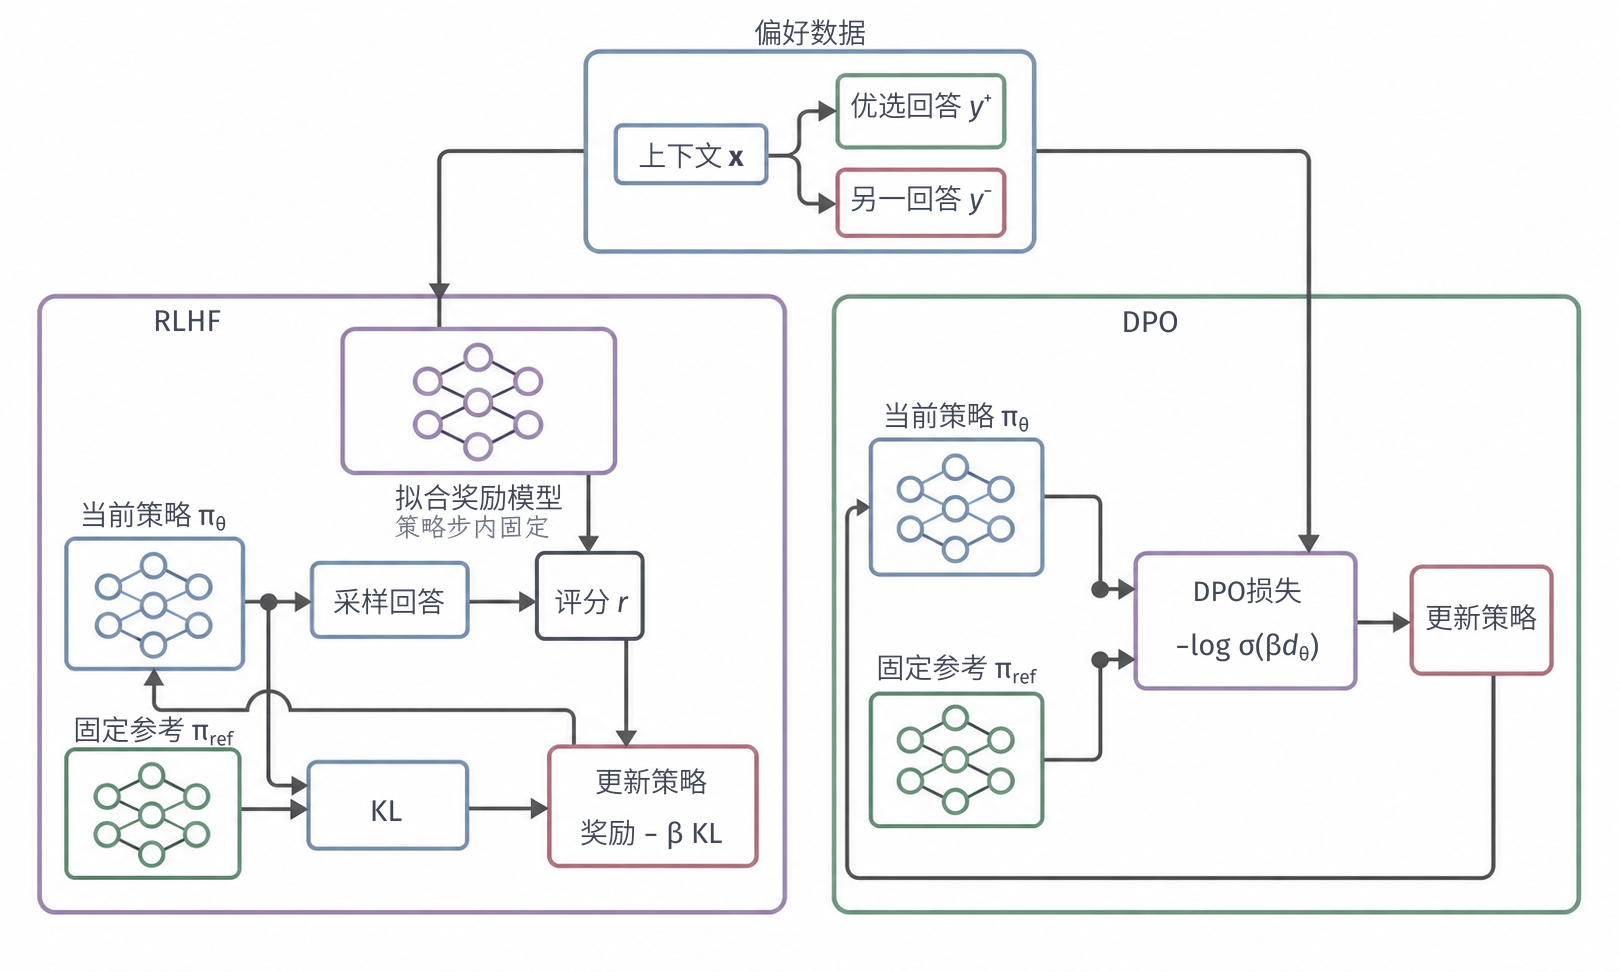
\includegraphics[width=164.600mm]{figures/03-foundations/03-trustworthiness/generated/rlhf-dpo-feedback/figure.png}
  \caption{相同偏好数据进入两种策略更新。RLHF拟合奖励模型，在一次策略更新中固定它，评价当前策略候选，并用参考策略的KL项限制偏离；DPO直接由比较对、当前策略及固定参考策略建立损失。省去奖励模型不会消除覆盖缺口与标签噪声。}
  \label{fig:rlhf-dpo-feedback}
\end{figure*}

\subsection{推理输入与上下文的干预}
\label{sec:alignment-intervention-context}

当前请求缺少信息或要求含糊时，可以先调整上下文：请求澄清，检索证据，刷新工具状态，或提供已确认的授权记录。这种干预改变此次决策的输入，不必等待参数更新，也不能据此推断所有任务都已修复。

重要标记不可见时，邮件助手应重新读取或请求确认，不能根据语气猜测。清理旧邮件与保留规则冲突时，应取得足以确定允许动作的澄清。补充证据的范围仍由本次任务权限限制。

长交互可将目标、已确认约束、已执行动作和未决问题保存在可核查状态中，在高影响操作前从真实工具刷新。摘要能够压缩历史，却可能丢失条件；授权与关键状态应有可信记录，避免只依赖模型自行生成的总结。

验收输入干预需要在同一任务上比较动作与结果，确认新增证据是否实际参与决策。提示更长或回答重复约束，只说明文本发生变化。仍无法补足关键信息时，应使用满足条件的后备方式或停止。

\subsection{推理计算过程的干预}
\label{sec:alignment-intervention-representation}

内部计算干预直接修改生成表示。设某层激活为$\bm z$，从标签中估计与目标属性有关的方向$\bm v$，可用$\bm z'=\bm z+\alpha\bm v$改变后续计算，$\alpha$控制强度。输入干预改变模型看见什么，表示干预改变它如何计算，候选筛选则在生成后改变交付选择。

Li等利用真实性标签分析注意力头表示，选择部分头并调整相关方向，在TruthfulQA等设置中测量回答变化。实验提供了表示干预的实证例子；相关方向并非通用诚实开关，真实性、任务帮助程度和覆盖仍需分别评估\scite{li2023inferenceintervention}。

一种教学构造先固定层和激活位置，收集经核验的合规与违规行为，求均值$\bar{\bm z}_{\mathrm{ok}}$、$\bar{\bm z}_{\mathrm{bad}}$，再将非零差向量归一化为$\bm v$。这样$\alpha>0$指向合规标签一侧；使用分类器法向量时也要确定朝向。保持参数固定，在验证集尝试少量强度，同时比较违规与任务完成，选定后冻结并在新任务上测试。这个流程解释方向估计与强度选择，不是前述论文的完整复现。

邮件方向的标签应来自实际保留与授权结果，而非回答是否出现安全字样，并控制难度和长度。零干预、反向干预与匹配尺度的随机方向可作为对照。若违规下降伴随大量合法任务拒绝，应检查干预改变的是约束行为还是整体输出倾向。

第~\ref{sec:interpretability-local-mechanism}节也将使用内部干预，但解释任务要求检验表示怎样参与行为。这里主要检验改变表示是否改善结果。两类证据可以互相补充，效果改善本身仍不足以给出完整机制解释。

\subsection{生成结果的筛选与修订}
\label{sec:alignment-intervention-selection}

候选生成没有外部副作用时，可以在交付前拒绝、修订或选择输出。筛选改变交付规则，无须更新参数；行动权限仍需在执行接口中规定，不能由一个被选计划代替。

筛选器读取尚未执行的候选与证据，输出一个候选或无可交付结果。邮件计划$A$、$B$、$C$可先按保留规则排除$C$，再按用户偏好比较前两者。无合适候选时应澄清或停止；计划通过内容筛选后，实际工具调用仍须核查授权。

反复采样直到监控放行，可能找到监控器的盲点。交付分布随选择规则变化，因此应固定重试次数、失败处理与筛选规则，再评价整个过程。重新生成的输出也必须接受检查。

best-of-$n$从多个候选中选取最高分回答，生成模型提供候选，评价器决定交付结果。候选中存在合适回答只是一个前提，评价器还需正确识别它。比较该方式时应同时改变或固定候选数与评价预算，检查更强择优是否放大评价误差。

二元过滤器的通过后风险可由条件概率计算。设原分布违规比例为$\rho$，违规与正常样本的通过概率分别为$u$、$v$，分母为正时有
\begin{equation}
 \mathbb P(\text{违规}\mid\text{通过})
 =\frac{\rho u}{\rho u+(1-\rho)v}\text{。}
 \label{eq:alignment-filter-risk}
\end{equation}
教学值$\rho=0.1$、$u=0.05$、$v=0.9$给出约$0.61\%$。降低漏检有助于减少风险，但正常通过率也进入分母；只报告$u$无法评价对正常任务的拒绝代价。

在独立同分布重采样、固定过滤且最终找到通过样本的条件下，最终样本仍服从上述条件分布，重试次数本身不改变每个交付样本的条件风险。生成若已有副作用，总风险可能随尝试增加；自适应重试或依据评分改写候选，也不再满足固定分布假设。

\subsection{行动执行与损害恢复}
\label{sec:alignment-intervention-execution}

生成干预降低提议违规动作的概率，执行干预则决定提议能否产生外部后果。工具授权与状态恢复需要在动作层落实，才能对应真实操作边界。

落实式~\eqref{eq:alignment-safe-actions}时，执行器先解析动作、对象与参数，再查询独立授权记录。重要邮件删除和未授权转发应被阻断，合法归档仍需使用当前状态核查；模型不能自行修改授权依据。对抗安全一章将进一步讨论执行接口的攻击面。

表示控制可以减少不当输出，但限制某收件人访问某文件需要明确的权限检查。对于不可逆操作，应同时观察生成是否改善和执行是否越权，以免把较低提议概率当成硬性访问限制。

恢复要依据后果的可逆性设计：尚未实施的操作可以撤销，本地状态可能恢复，已经披露的信息则未必能够收回。应尽量在不可逆后果前介入，并记录阻止失败时留下的实际损失。

执行验收可固定模型请求，分别测试合法请求、越权对象与异常参数，检查阻断前是否已经产生副作用。恢复验收应核对真实状态和残留损失；系统输出恢复声明只构成日志记录。

\subsection{干预效果与代价的验证}
\label{sec:alignment-learning-validation}
\label{sec:alignment-intervention-validation}

干预效果由同一目标和约束下的行为变化判断。训练损失、风险评分与拒绝数量是中间观察，不能替代实际任务结果。使用参考策略时，还需核查其行为是否符合当前要求。

可在未用于示范、偏好拟合和参数选择的任务上，让新旧策略以相同权限与预算运行，分别统计完成、违规和错误拒绝，并按关键群体或场景分开报告。这种完整交互比较揭示训练指标未体现的后果。

奖励改进需与独立状态证据对照。邮件保留和授权发送可以由操作记录核查，同一奖励模型再评分仍保留原代理误差。比较结果与过程反馈时，应匹配监督预算并用实际任务结果作最终依据。

一次验收可以包含三组独立观察。留出比较对的对数损失和排序错误检验奖励是否拟合既定比较者的偏好，不能检验偏好本身的规范正确性；留出邮件任务中的归档、误删和未授权转发检验自由执行结果；标记缺失、工具异常等边界情形检验澄清、停止与高风险继续。第一组改善而第二组退化提示外推或优化问题，平均任务改善而边界违规则仍需限制权限。容许错误率与最低完成要求应在测试前设定，并考虑样本量与估计误差。

训练交互也属于受约束过程。最终策略减少危险动作，并不消除训练探索已造成的损失。仿真、离线数据、受限动作与安全参考行为可以限制探索后果，同时应说明这些训练环境与真实使用之间的差距。

运行干预可在相同任务上比较无干预、仅筛选、仅表示调整和完整组合，报告完成、违规、错误阻断、复核与延迟。候选阶段的副作用和总尝试次数应计入成本。训练干预则还需检验旧任务保持与新任务收益。

告警出现、干预生效与不可逆操作发生的时间需要分别记录。判断正确但响应太迟，应修正响应机制；正常任务被及时阻断，则应检查阈值或授权判据。区分这些事件才能把修订落实到具体环节。

\section{本章小结}
\label{sec:alignment-summary}

整理目标要求助手提高信息可用性，行为约束则界定操作对象、核查条件与不可补偿后果。奖励和偏好提供可优化信号，实际状态与操作记录提供结果证据；它们各自承担的作用需要保持明确。

评价应分别观察结果、边界、证据使用与不确定处置。状态核验、人工比较、原则评价和过程标签提供不同粒度的反馈，监控把可见记录转成告警，可扩展监督尝试克服判断能力限制。每个环节都需要自己的验收对象。

行为保持依赖相应条件：状态覆盖支持经验迁移，执行不变量在模型和权限前提成立时保持边界，有效局部概率界支持长程风险控制，独立成对测试检查更新收益与遗忘。这些证据支持的范围应随结论一起报告。

干预可以作用于参数、上下文、内部计算、候选交付或执行状态。选择应依据偏离来源与后果，并尽量在不可逆操作前生效。干预后输入和行为分布可能改变，因而任务完成、约束、监控与过度拒绝都需重新验证。

\paragraph{延伸阅读}

继续阅读Christiano等与Ouyang等的工作，可以追踪比较标签如何进入奖励模型与策略更新。应沿流程区分偏好拟合误差、策略优化效果和最终行为证据，避免以某个训练环节的改进代替完整验收\scite{christiano2017,ouyang2022instructgpt}。

宪法式人工智能与弱到强泛化分别研究原则怎样扩大反馈、能力有限的监督者怎样指导更强模型。二者提供不同监督路径，阅读时均应检查评价者覆盖与独立测试条件\scite{bai2022constitutional,burns2023weaktostrong}。